\pagestyle{empty}
%\ifpdf\mbox{}\else
\begin{center}
%\centerline{\rule{\textwidth}{0.3mm}}
%\vfill%\vspace{4cm}
\vspace*{4.cm}
{\Huge \bf M\'{e}todos Estat\'{\i}sticos em


\vspace*{0.8cm}
F\'{\i}sica Experimental}


\vfill%\vspace{3cm}
%{\LARGE \bf \it Mauro Anselmino}\\*[2em]
%{\LARGE \bf \it Francisco Caruso}\\*[2em]
%{\LARGE \bf \it Jos\'{e} Roberto Mahon}\\*[2em]
%{\LARGE \bf \it Vitor Oguri}\\

%\vfill
%\includegraphics[width=4.3cm]{Fig/ABDR-logo-PB}
\end{center}%
	%
%\cleardoublepage
\newpage


\vspace*{5.0cm}
\thispagestyle{empty}
\centerline{}

%\begin{center}
%\centerline{\rule{\textwidth}{0.4mm}}
%\end{center}
%\fi
%\vfill%\vspace{4cm}
%\newpage
%\cleardoublepage
	%
%\begin{center}
%\centerline{\rule{\textwidth}{0.3mm}}
%\end{center}
%\fi
%\vfill%\vspace{4cm}

\newpage
\vspace*{2cm}
\begin{center}
{\Huge \bf M\'{e}todos Estat\'{\i}sticos em


\vspace*{0.8cm}
F\'{\i}sica Experimental}

%{\Huge \bf Introdu\c{c}\~{a}o \`{a} QCD Perturbativa}\\*[1.5em] {\Large (d\'{e}cima vers\~{a}o corrigida)}
%\vfill
\vspace{2cm}
{\LARGE \bf \it Vitor Oguri}\\*[1.5em]
{\large {Departamento de F\'{\i}sica Nuclear e Altas Energias \\ Instituto de F\'{\i}sica Armando Dias Tavares\\ Universidade do Estado do Rio de Janeiro (UERJ)}}
%{\large \bf Rio de Janeiro}

\vfill
%\includegraphics[width=3.5cm]{Fig/Gen-LTC-logo}
\end{center}
%\ifpdf
%\begin{flushleft}\protect
%\tableofcontents\protect%
%\end{flushleft}\protect
%\fi
%%\cleardoublepage%\newpage
	%
%% \chapter*{}\mbox{}%\mbox{~}\vskip7cm
%%\thispagestyle{empty}
%\\\ vfill
%%\mbox{ ~ } \hfill
%
%\vfill
%%\mbox{\phantom{m}} \\
%%\mbox{}
%\clearpage \thispagestyle{empty}

\newpage
\thispagestyle{empty}

\vspace*{-3cm}

\centerline{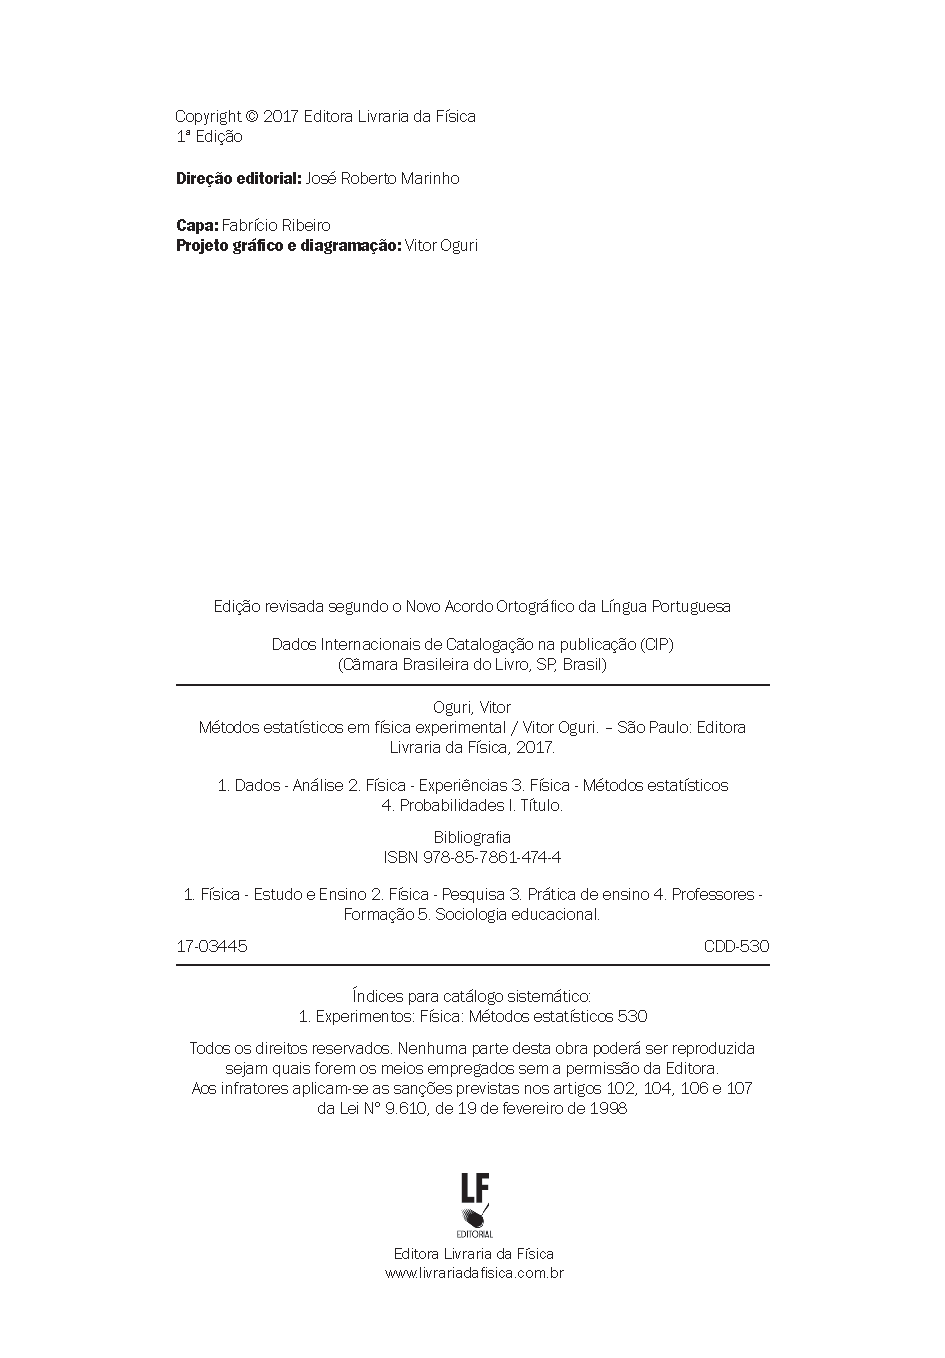
\includegraphics[height=23cm]{ficha_catalografica}}

\newpage

%\setcounter{page}{0}

\begin{flushright}
\begin{minipage}{3.cm}
\baselineskip=8pt
\hfill A Nobuo Oguri, \textit{in memoriam}

\end{minipage}
\end{flushright}

\vspace*{5.cm}
\begin{flushright}
\begin{minipage}{6.5cm}
\baselineskip=8pt
\textit{Se deseja saber a ess\^{e}ncia do m\'{e}todo cient\'{\i}fico, n\~{a}o preste aten\c{c}\~{a}o ao que lhe possa dizer um cientista. Observe o que ele faz.}
\medskip

\hfill {Albert Einstein}
\end{minipage}
\end{flushright}

%===============================================================
%\input{prefacio_oguri}
%\setcounter{chapter}{-1}
%\cleardoublepage%
%===============================================================
\chapter*{Pref\'{a}cio}
%===============================================================
%\ifpdf\relax\else
%\pagestyle{fancy}
%\fi
\addcontentsline{toc}{chapter}{Pref\'{a}cio}%
\markboth{Pref\'{a}cio}{Pref\'{a}cio}%

\baselineskip=14pt

\vspace*{-0.7cm}
\paragraph*{}
Este livro \'{e} fruto da experi\^{e}ncia do autor em an\'{a}lise de dados em experimentos de F\'{\i}sica, desde  sua forma\c{c}\~{a}o inicial nos anos de 1980, na \'{a}rea de raios X e radia\c{c}\~{a}o s\'{\i}ncrotron, nos laborat\'{o}rios  da faculdade de engenharia f\'{\i}sica da Universidade de T\'{o}quio e na {\it Photon Factory} do KEK,\footnote{Acelerador  S\'{\i}ncrotron do  Laborat\'{o}rio de Altas Energias do Jap\~{a}o, em Tsukuba.} at\'{e} a sua participa\c{c}\~{a}o em  grandes experimentos de Altas Energias; DZero  do Fermilab\footnote{Fermi National Accelerator Laboratory, Batavia, Illinois, USA.}  e CMS do CERN,\footnote{Centro Europeu de F\'{\i}sica de Part\'{\i}culas, Genebra, Su\'{\i}\c{c}a.} nos anos de 1991 at\'{e} 2013.

 O material selecionado \'{e} abordado no corpo do texto de modo intuitivo, es\-pe\-ran\-do-se que o leitor tenha familiaridade apenas com os t\'{o}picos b\'{a}sicos de um curso de C\'{a}lculo Diferencial e Integral,  e com alguns conceitos da Estat\'{\i}stica,  todos temas abordados regularmente nos ciclos b\'{a}sicos dos cursos de F\'{\i}sica, Qu\'{\i}mica  e Engenharias.

O texto que serviu de ponto de partida do livro corresponde \`{a}s notas de aula da disciplina de Tratamento estat\'{\i}stico de dados em F\'{\i}sica, mi\-nistrada pelo autor em diversos per\'{\i}odos, ao longo dos \'{u}ltimos 10 anos, na gradua\c{c}\~{a}o e no programa de p\'{o}s-gradua\c{c}\~{a}o do Instituto de F\'{\i}sica Armando Dias Tavares da  Universidade do Estado do Rio de Janeiro (Uerj).
	
Apesar de muitos exemplos serem tomados da \'{a}rea de Altas Energias, as ferramentas e os  m\'{e}todos estat\'{\i}sticos apresentados podem ser utilizados em qualquer experimento que envolva processos aleat\'{o}rios.

O autor agradece aos colegas do Departamento de F\'{\i}sica de Altas Energias da Uerj, Alberto Franco de S\'{a} Santoro, Francisco Caruso, Jos\'{e} Roberto Mahon e Dilson de Jesus Dami\~{a}o, pela leitura, cr\'{\i}ticas  e sugest\~{o}es ao texto.

Um agradecimento especial \`{a} Stella Maris Amadei pela cuidadosa  leitura de diferentes vers\~{o}es de todos os  cap\'{\i}tulos e pelas sugest\~{o}es de estilo.


\vspace*{0.2cm}

%\leftline{\textit{Rio de Janeiro}}

%\vspace*{0.3cm}
\rightline{\textbf{V.O.}}
%\clearpage
%\par
%\vfill

\newpage \ \\
\thispagestyle{empty}



%===============================================================
% \newpage
% \thispagestyle{empty}
% \ \\
%===============================================================
%\input{apresentacao}
%===============================================================

%\ifpdf\relax\else
\begin{flushleft}\protect
\tableofcontents\protect%
\end{flushleft}\protect

\vfill

%\newpage

\endinput
%===============================================================
